\section{Infrastructure and Monitoring Systems}
\label{sec:slow-control}

MicroBooNE is housed at LArTF, which is located on-axis to the BNB.  Complete knowledge of the electrical and cryogenic systems housed within LArTF is necessary to maintain acceptable operating conditions for the experiment.  Continuous monitoring of the beam being delivered to LArTF is also necessary for subsequent physics analyses.  This section describes the details of infrastructure within LArTF, as well as monitoring of the experiment and beam conditions.

%\subsection{Infrastructure}
%{\it{Suggestion from Bryce and Linda}}
%Brief Intro\\
%- AC Power Distribution for Low-Noise and Conventional Electronics\\
%-- Discuss saturable inductor and clean power/ground, characteristics of clean power circuits\\
%-- Describe which subsystems are on clean or building ground.\\
%-- Describe ground monitor\\
%-- Describe AC distribution on platform and in rack (on rack cabling, AC distribution boxes, PDUs, RPS intl'k, etc)\\
%
%FIGURE: Illustrative line drawing (not complete drawing) of AC distribution
%
%PHOTO: Ground monitor, saturable inductor, in-rack AC distribution
%
%- DC Power Distribution to TPC\\
%-- Describe DC power distribution to TPC electronics and TPC: MPOD, PL508s, D0 supply for HV\\
%-- Give general delivered powers/currents\\
%- Network and Data Cabling Scheme\\
%-- Describe how network is sent to platform racks\\
%-- Describe how data is transferred to DAQ machines\\
%-- Briefly mention timing, calibration, trigger, clock, config signals/fanout, which are described in sub-system sections.\\
%-- Describe cable shielding methods (copper in cables trays, etc. etc.)\\
%-- Discuss mapping generically (maybe not the full gritty details)\\
%
%FIGURE: Illustrative line drawing of Signal/Network distribution
%
%- Interlocks and Safety Systems\\
%-- Discuss fire protection\\
%-- Discuss temperature monitoring\\
%-- Discuss existing hardware interlocks\\

\subsection{Electronics Infrastructure at LArTF}
\label{sec:lartf}


The electronics infrastructure of the experiment, which is essential for proper operation of the electronics that control the functioning of and extract data from the LArTPC, PMTs, and other detector systems.  Figure~\ref{fig:ElecInfDiagrams} shows a diagram of this system at LArTF, depicting racks located on a platform directly above the cryostat that house electronics for: \lartpc control and readout, light collection system, drift high voltage, purity monitor, calibration laser, trigger, and cryogenic control systems.  Additional server racks containing the DAQ servers, beam timing, and external network electronics are located in a separate computer room above and adjacent to the above-cryostat platform.  The distribution of power, data, and network connections to and from all of these racks is also presented in figure~\ref{fig:ElecInfDiagrams}, and is described in more detail in the following sections, as are electronics safety systems and interlocks.

\begin{figure}
\centering
\includegraphics[width=0.8\textwidth]{./figures/ACDist.png}
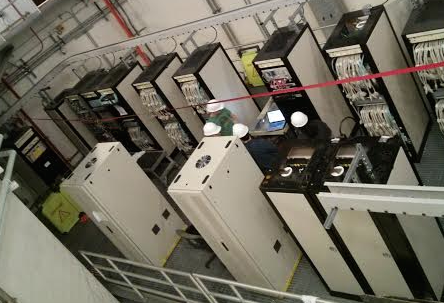
\includegraphics[width=0.6\textwidth]{./figures/ActualRacks.png}
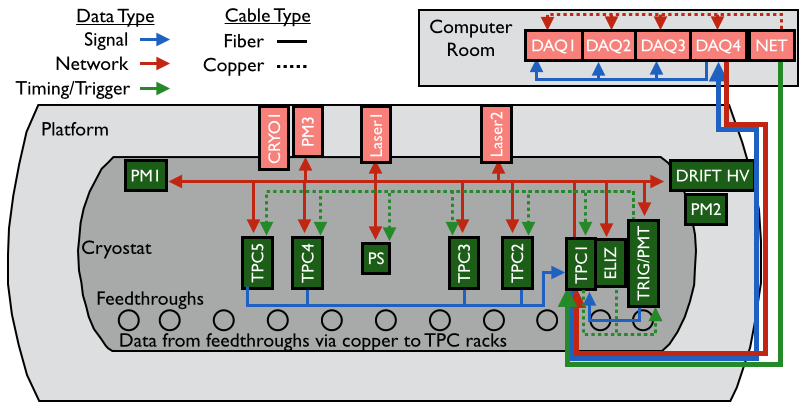
\includegraphics[width=0.8\textwidth]{./figures/DataDist.png}
\caption[]{Top: Diagram illustrating location of deployed electronics racks and separation of detector and building grounds and clean and building power for differing racks.  Middle: Photograph of installed electronics racks on the LArTF platform.  Bottom: A diagram illustrating the general scheme of signal, network, and timing signal cabling in the LArTF computer room and platform.}
\label{fig:ElecInfDiagrams}
\end{figure}

\subsubsection{AC Power Distribution and Grounding for Low-Noise LArTF Data-taking}
As with any large detector operating with a high dynamic range, prevention of electromagnetic interference and its attendant effects on MicroBooNE data is an essential aspect of detector design.  MicroBooNE's strategy for producing a low-noise environment for the \lartpc and associated readout electronics can be largely summarized in a few key points.  AC power distribution-related items will be described here, while cabling, connections, and shielding will be described in a following section.

\begin{itemize}
\item{``Clean power,'' or AC power electrically isolated from AC power for the rest of LArTF (``building power''), is supplied to all sensitive electronics via an isolation transformer.}
\item{Highly sensitive electronics are housed inside the Faraday cage provided by the detector cryostat or inside Faraday cages directly grounded to the cryostat.}
\item{The detector cryostat is grounded to a ``detector ground,'' which is physically and electrically isolated from the ground provided to all other LArTF power circuits, or ``building ground.''}
\item{No direct electrical connections are present between detector ground and building ground.  This is accomplished through the use of insulating platform and cryostat saddle materials, insulating cable trays and cables, and by inserting insulating ``breaks'' (i.e. fiber data links or insulating cryo pipe sections) when connections between sensitive and potentially noisy detector components are necessary.}
\item{Indirect pickup on clean signals through capacitive coupling to adjacent noise sources is minimized through use of detector-grounded shielding and electrically-insulating cable trays.}
\item{Ground loops on detector ground are avoided wherever possible by connecting all electronics racks directly to the cryostat and by minimizing direct electrical connections between racks.}
\item{Direct or capacitive couplings between building and detector ground are constantly monitored during installation and operation with a custom-designed impedance monitor.}
\end{itemize}

A line drawing describing the production of clean power and clean ground is shown in figure~\ref{fig:ElecInfAC1}.  A pair of 200 A clean power circuits produced at isolation transformers are used to power all sensitive racks, which are indicated in figure~\ref{fig:ElecInfDiagrams}.  All racks containing \lartpc readout electronics are placed on one circuit, while all other sensitive equipment is placed on the alternate circuit.  On the platform, all racks utilize clean power with the exception of the calibration laser and in-line purity monitor racks, which either contain noise-producing elements or support building-grounded components.  All racks in the LArTF computer room utilize building power.

\begin{figure}
\centering
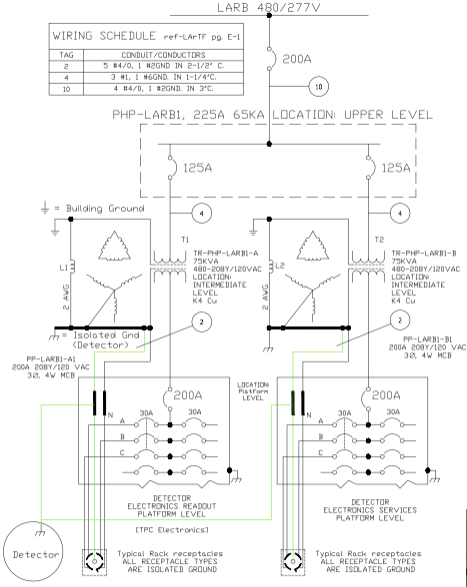
\includegraphics[width=0.55\textwidth]{./figures/PowerDiagPic1.png}
\caption[]{Line drawing of clean power generation and distribution and connections to detector ground.}
\label{fig:ElecInfAC1}
\end{figure}






The 208 volt, 3-phase power is distributed to each individual electronics rack.  For racks with significant power requirements or a large number of components, this power is delivered to a Fermilab-designed ``AC switch box,'' which distributes power to an Eaton Power Distribution Unit (PDU) only upon receiving an interlock signal from a smoke detection system in each rack, which will be described in more detail below.  Rack components then receive power from one of the three phases on this PDU.  For racks with fewer requirements, power is supplied to components directly from an interlocked simplified AC switch box or SurgeX SX-1120-RT PDU.  Racks with sensitive electronics are grounded to the cryostat via copper sheeting running throughout insulated cable trays above the cryostat.  Sensitive components within each rack are connected to a tin-plated copper grounding bar electrically connected to the rack bottom and running the height of the rack.  Mechanical attachments to the rack provide grounding for less sensitive rack components.  As mentioned before, any unintentional direct connection between building and detector ground can be quickly identified by the impedance monitor located on the LArTF platform.  Figure~\ref{fig:ElecInfAC2} shows photographs of this equipment.

\begin{figure}
\centering
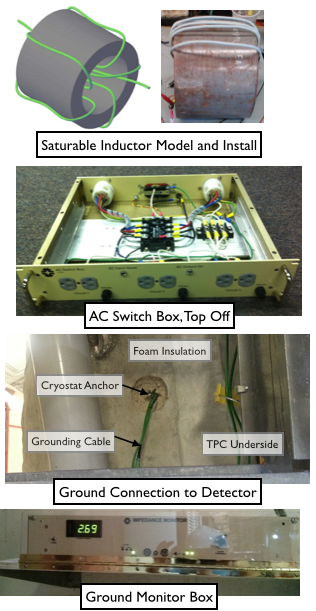
\includegraphics[width=0.55\textwidth]{./figures/PowerDiagPic2.png}
\caption[]{Photographs of the installed saturable inductor (top), AC switch box (top middle), detector ground strap and connection (bottom middle), and impedance monitor (bottom).}
\label{fig:ElecInfAC2}
\end{figure}


%FIGURE/photo: Illustrative line drawing (not complete drawing) of clean power generation and grounding; Saturable inductor, grounding hub, in-rack AC distribution

\subsubsection{DC Power Distribution to the MicroBooNE Detector}
DC power is provided to the \lartpc and readout electronics by power supplies in clean-powered, detector-grounded racks for a variety of purposes including
\begin{itemize}
\item{Holding the \lartpc cathode plane at voltage to produce the desired ionization electron drift speed.}
\item{Holding the two ungrounded anode planes at the proper constant voltage to ensure the planes are transparent to drifting electrons.}
\item{Operating the light collection system PMTs.}
\item{Powering the cold electronics located inside the \lartpc.}
\item{Powering the warm electronics located in the \lartpc and PMT readout electronics racks}
\item{Powering auxiliary systems, such as purity monitors.}
\end{itemize}

Table~\ref{tab:DCPower} summarizes the required voltages or currents for each of these purposes as well as the power supply make and model utilized in each case.  Power supplies are located in the relevant subsystem's electronics rack, with power and grounding connections as dictated by that rack.

\begin{table}[!htb]
	\centering
	  \caption{Overview of MicroBooNE DC power distribution.  Delivered voltages or currents are listed, along with power supply makes and models and whether each supply utilizes clean or building power.}
    \begin{tabular}{llll}
     \hline
      System & Supplied Value & Supply Make/Model & Clean Power? \\ 
      \hline
      Drift High Voltage & 120 kV & Glassman LX150N12 & Y \\ 
      \hline
      Wire Plane Voltage & $\pm$1 kV / 8 mA & Wiener MPOD  & Y \\ 
  %    & & ISEG$\_$EHS 82 10X$\_$805F  &\\ 
      \hline
      PMT High Voltage & 2 kV / 3 mA & BIRA T4 & Y \\ 
      \hline
      Cold Electronics Power & 8 V / 10 A & MPOD MPV 800l & Y \\ 
      \hline
      Warm LArTPC/PMT& +/-5 V MDH 2-8 V/25 A& Wiener PL508 & Y\\
       Electronics & +12 V MEH 8-15 V/92 A & & \\ 
      & +3.3 V MEH 2-7 V/115 A & & \\ 
      \hline
       Auxiliary Systems & Various & Various & Laser: N \\
      Power &&& Inline PM: N \\
      &&& Cryostat PM: Y \\ 
      \hline
  \end{tabular}
  \label{tab:DCPower}
\end{table}

DC supply power consumption is minimal in most cases, with the exception of the warm \lartpc electronics PL-508 supplies.  Care was taken to distribute the AC power load by limiting the number of high-draw PC supplies per electronics rack.

\subsubsection{Network, Timing, and Data Distribution for Low-Noise LArTF Data-taking}

Network, timing, and data connections must be made between the detector, building-ground, and detector-ground racks to properly read out MicroBooNE data.  However, as described above, these connections must be made while maintaining strict detector-building electrical isolation.  Deployed interconnections meeting both of these requirements are displayed in figure~\ref{fig:ElecInfDiagrams}.

Timing and LArTF-external network signals are brought into LArTF via electronics in the computer room, where all racks are building grounded and powered.  These signals are distributed and processed in the computer room via copper cable, while network and processed timing signals to be sent to the platform are converted onto fiber cables and aggregated into a central fiber termination box.  A fiber trunk line then delivers these signals to the platform, where another fiber termination box on a detector-ground rack is used to fan out these signals.  Network connections are fanned out via fiber to a network switch in each platform rack, while timing signals are re-converted to copper and further processed for use by the trigger system on a different detector-grounded rack.  All rack-to-rack cables are run in insulating cable trays beneath the platform.

PMT and \lartpc data are transferred from each detector feedthrough to readout crates in detector-ground racks via insulated copper cable whose shield is tied to detector ground.  Digitized crate output is then sent to the aforementioned platform fiber termination box, where these signals are sent via fiber trunk line to the computer room.  In the computer room, these fibers are then fanned out to the appropriate DAQ computer.  Readout crate and cold electronics control commands are transmitted in the opposite direction utilizing a similar scheme, with crate controls delivered directly via fiber, and cold electronics commands delivered via fiber to a copper fanout in a detector-ground rack.

Clock and trigger signals must also be sent from a central trigger rack to all detector-ground LArTPC/PMT readout racks.  These signals are transmitted via copper connections, and represent the only source of ground loops on detector ground.  To further reduce the possible impact of induced noise in these and all copper cables mentioned above, all insulating cable trays beneath the platform are lined with copper sheeting grounded to the detector.  As an additional precaution, all \lartpc signal copper cables are run in separate cable trays from power and auxiliary cabling beneath the platform as well as inside every rack.

All cables between all detector components have been uniquely labelled with serial number, source, and destination to allow for ease of replacement and reconnection.  Ample fiber and copper spares for every major cable type are also installed along with the production cables to allow for quick replacement of any failed cable.

\subsubsection{Interlocks and Safety Systems}
All electronics racks contain smoke-sensing and temperature-monitoring systems, which, when interlocked with AC and DC power transmission in each rack, constitute a rack protection system (RPS) designed to meet Fermilab safety requirements and reduce the risk of fire and related damage in LArTF and to individual rack components.

The RPS principally consists of a smoke sensor connected to a Fermilab-designed rack protection box.  This box produces and outputs a 12~V interlock signal when the rack protection box is on and receiving a ``no-smoke'' signal from the smoke sensor.  This 12~V signal can be sent to the AC distribution box located in each rack, as described above, to allow AC transmission to all rack components only if the RPS is on and not detecting smoke.  A similar 12~V ``RPS Status'' signal is also produced by the RPS box for input into the MicroBooNE slow control box, which will be described in following sections.  Alternate contacts are available on the rear of the RPS box for coupling the status of additional subsystems, such as the DAQ and calibration laser uninterruptible power supply (UPS), to smoke sensor or rack power status.

Temperature sensors deployed in two or three locations in each electronics rack sample air temperature within each rack.  Temperatures at each sensor are read out and recorded in the slow-control database by the slow-control monitoring box.  In addition, the box also produces a 5 V interlock signal if all sampled temperatures are within pre-programmed thresholds.  In electronics racks distributing PMT- or LArTPC-related DC power these temperature interlock signals are input into each relevant power supply, allowing DC power distribution only when this interlock signal is present, for safety purposes.

Additional hardware interlocks ensure the non-simultaneous operation of particular systems.  In particular, the PMT system is disabled when cryogenic system liquid level sensors detect a level below that of the highest PMT bases, or when the UV laser system is active.  The former requirement is enforced with a dry-contact hardware interlock, while the latter is enforced with a software interlock in the MicroBooNE online software.  The UV laser system is also dry-contact hardware interlocked.  Finally, the HV drift power supply is directly interlocked with the cryogenic system controls liquid-level sensor via a dry-contact hardware interlock.

\subsubsection{Performance Measurements}

The proper operation of each production electronics rack's AC and DC distribution and RPS systems has been tested prior to installation at LArTF.  Furthermore, test stands exercising functionality of DAQ, PMT and \lartpc electronics, trigger, and drift HV systems have successfully incorporated and tested various aspects of these same AC and DC distribution and RPS systems.  Impedances between detector and building grounds were recorded throughout the installation of the rack infrastructure at LArTF using the impedance monitor located on the LArTF platform.  %BRIEF OVERVIEW OF RESULTS OF IMPEDENCE TESTS.



\subsection{Slow monitoring and control system}
%{\it{(Slow controls team: Glenn, Sowjanya)}}

% Definition, scope of functionality, and software products
MicroBooNE uses EPICS for controlling and monitoring most devices and conditions important to the experiment.  These include power supply controls, temperatures, fan speeds, rack protection interlock status, and various environmental conditions.  The DAQ, cryogenics systems, and beam data collection systems operate independently of the EPICS slow monitoring, but export data which are imported into EPICS for archiving and status displays.  Applications from the Control System Studio software collection \cite{ControlSystemStudio} are used for providing displays, alarm notifications, and data archiving.

\paragraph{EPICS architecture}
% Controllers
An EPICS system consists of any number of server programs implementing the EPICS Channel Access (CA) protocol \cite{EPICS_CAP_Spec} to provide client programs access to any number of process variables, where each process variable represents a quantity being controlled (an output) or measured (an input).  The EPICS base distribution provides a standard type of channel access server called an Input/Output Controller (IOC), which can be extended to support specific hardware as desired.

\paragraph{Power supply controls}
% Power supplies: Wiener, PMT, and Glassman
Most power supplies are controllable over the network through the NetSNMP protocol \cite{NetSNMP}.  Several EPICS driver modules are available for SNMP, and MicroBooNE utilizes one written at NSCL \cite{devSNMP}.  An IOC with this SNMP module runs on a central computer and contacts the power supplies over a private network for monitoring and control.  The photomultiplier power supplies are reused from the D\O\  experiment and have custom IOCs running in their own controllers.  The main high voltage power supply has only a simple RS-232 serial interface; control and monitoring for it is provided by a nearby computer running an IOC with the EPICS asynDriver \cite{asynDriver} and StreamDevice \cite{StreamDevice} modules.

\paragraph{Slow controls box}
% Custom hardware
MicroBooNE has a number of racks in various positions above the detector and in an adjacent server room.  Each is equipped with a rack-protection system and multiple digital temperature sensors, and most contain one or two fan packs, each containing 6 fans.  To monitor and control these devices, each rack has an 1U rack-mount enclosure containing an ARM-based single-board computer (SBC) running Linux and a custom interface board, collectively known as a "slow controls box".  An off-the-shelf GESBC-9G20 from Glomation Inc.~\cite{GlomationInc} is utilized for the SBC.  The custom interface board \cite{HuffmanFanInterfacePage} connects the SBC to front panel LEDs, temperature probes, fan packs, and rack-protection-status input. The temperature sensors are DS1621 chips, controlled and read out over an I2C bus by the SBC's I2C controller.  The DS1621 also has a thermostat output with programmable trip and reset temperatures, which are connected via the interface board to outputs that can be used to interlock devices in the racks, such as power supplies.  The fans provide pulse-per-rotation outputs, which are monitored by a 12-channel tachometer implemented via a PIC16F887 microcontroller, and also read out by the I2C bus.  An EPICS IOC runs in each SBC, with custom device drivers for reading all status information and controlling the heartbeat LED and temperature sensor trip and reset points.

\paragraph{External data sources}
% Data importers
Data are imported into EPICS channels from a number of external sources. The primary reason for duplicating these data in EPICS is to integrate displays and warnings into one system for the experiment operators, and to provide integrated archiving for sampled data in the archived database. An IOC running on a central computer provides ``soft'' process-variables channels for these data.  The data acquisition system provides many metrics describing its operation via the Ganglia system\cite{GangliaBook,GangliaHomePage}, which makes the data available in an XML format easily read by a Python script, which in turn writes to EPICS using the PyEPICS module \cite{PyEPICS}.  The hardware and system status of the DAQ computers is monitored through the industry standard Intelligent Platform Management Interface (IPMI); rather than writing a script to import data from IPMI directly into EPICS, a IPMI-to-Ganglia interface provided by the FreeIPMI's ``ipmi-sensors'' package \cite{FreeIPMI} is used, allowing data to be imported via the same mechanism used for the DAQ metrics.  Separate Python scripts periodically retrieve data about outside weather conditions from various sources, cryogenics system data from a file retrieved non-intrusively from the IFIX cryogenics control system, and beam data from Fermilab's Intensity Frontier Beam Database (IFDB) \cite{IFBeamDB}. 

%Beam monitoring
\subsection{Beam Monitoring}
%{\it{Zarko Pavlovic, Tom Kobilarcik}}
\label{sec:beam-monitoring}

The primary source of neutrinos for the MicroBooNE experiment is the BNB.  NuMI beam data is also recorded on a spill-by-spill basis.  The primary beamline is lined with instrumentation including toroids which indicate beam intensity, ``multiwires'' showing beam profile in the horizontal and vertical planes, and beam position monitors measuring the mean beam position. Data from these monitors are stored on a spill-by-spill basis in the IFDB. Many of MicroBooNE's physics analyses require that beam data are recorded for each spill and matched to detector events.

Primary beam monitoring in MicroBooNE is done using a ``dashboard'' interface to IFDB. By using the IFBD instead of the accelerator control system, the experiment can also verify that data are being acquired by the IFBD. The dashboard is accessible over the network using a web browser. The final monitoring step includes a post-data-merge check, ensuring that beam data are successfully matched with detector data for all beam spills. This is done once the detector DAQ binary data file is closed. 

The dashboard presents a graphic representation of the data, allowing for easy error identification, as shown in figure \ref{fig:beammonitor}.  The experiment monitors two toroids, which indicate beam intensity; three multiwires, each of which shows beam profile in each plane; and beam position monitors along the beamline, which show the vertical and the horizontal position.  Parameters pertaining to the target and horn, such as cooling air temperature and horn current, can also be monitored.  The dashboard allows the experiment to easily add additional devices if experience demonstrates the need for their monitoring.

Data are monitored in near real-time.  A reasonable history is also kept so that changes are easily identified.  The accelerator control system provides detailed diagnostics tools to experts and can be used in case of any problems.

%(We do not have a good way to monitor the secondary beam -- is this worth elaborating?)

\begin{figure}
\centering	
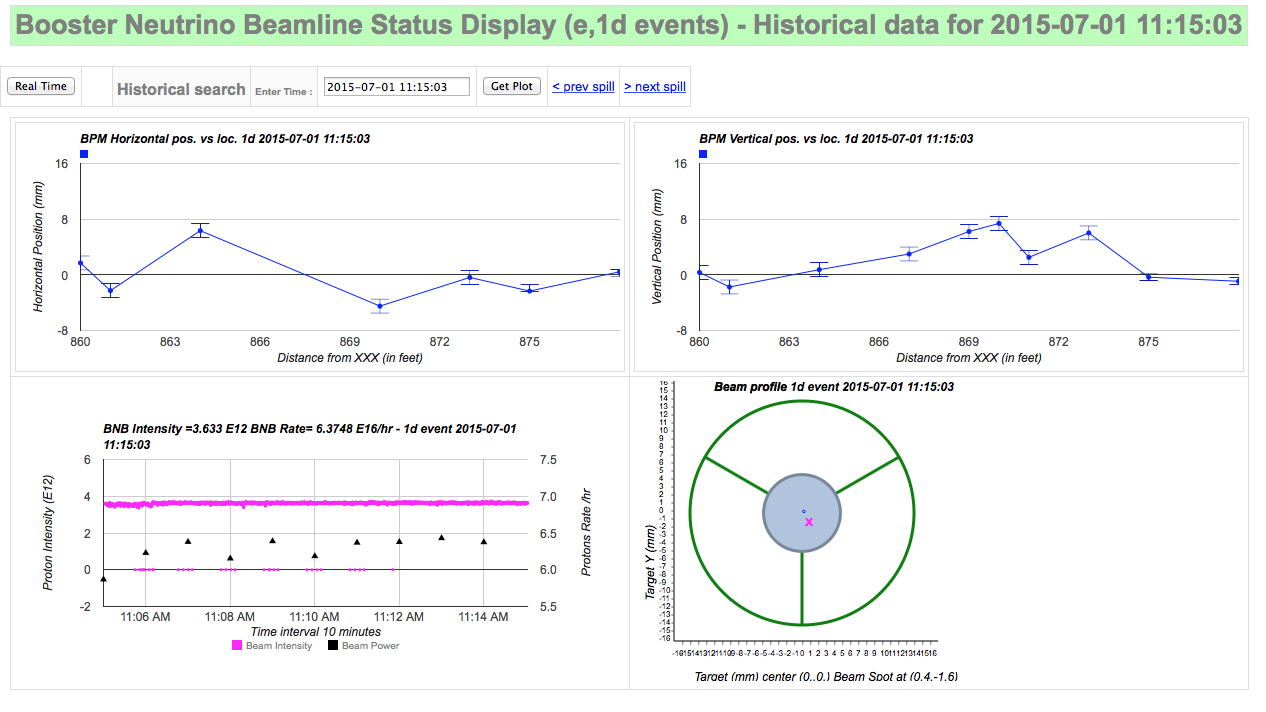
\includegraphics[width=0.95\linewidth]{figures/beam_monitoring.png}
\caption{The BNB dashboard, showing graphical representation of beam instrumentation data, is used to monitor the beam. The top box shows the timestamp of the beam spill and indicates if data is stale by changing the color. The two top plots show the primary proton beam position along the BNB. The bottom left plot shows the recent beam spill intensity and rate. The bottom right plot shows the beam as projected onto the Beryllium target (the grey circle in the middle with radius of 0.5~cm). The dashboard is accessible via web page providing both real time updates and the review of past data. The page can be easily extended to monitor additional beam devices.}
\label{fig:beammonitor}
\end{figure}


